\subsection{Niveau 2 - Pulveriser}

\begin{center}
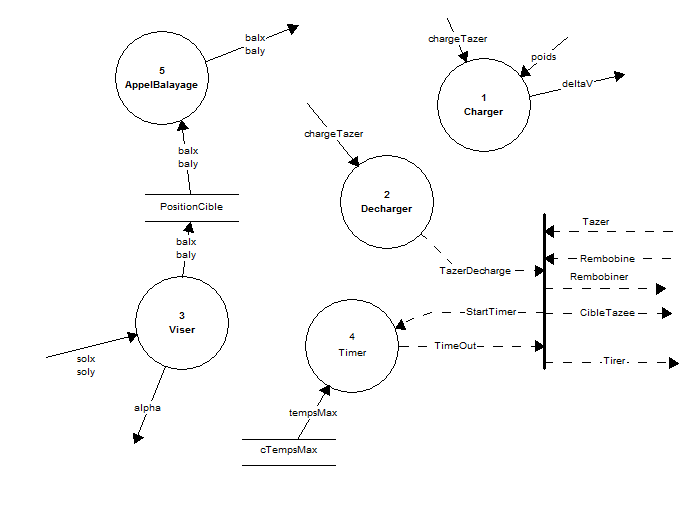
\includegraphics[scale=0.8]{\PIXPATH/tazer}
\end{center}


\subsubsection{Diagramme état-transition}

\begin{center}
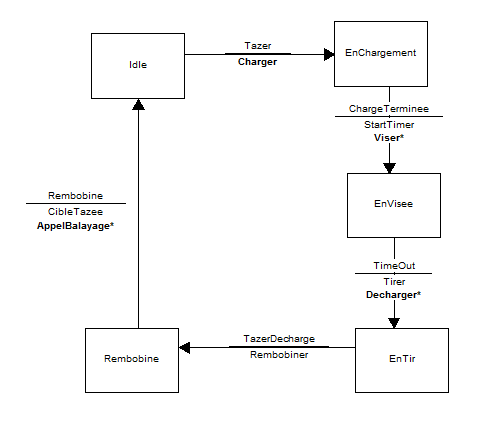
\includegraphics[scale=0.8]{\PIXPATH/tazer_etat}
\end{center}

\vfill
\pagebreak

\subsubsection{Processus primitifs - C-Spec}

\begin{description}
	
	\item \textbf{Orienter}
		\begin{tabbing} 
		\textbf{IN} : x, y, z, Orienter \\
		\textbf{OUT} : angle1, angle2 \\
		angle1 : $\arccos{\frac{x}{\sqrt{x^2+y^2}}}$ \\
		angle2 : $\arccos{\frac{z}{\sqrt{x^2+y^2+z^2}}}$ \\
		Orienter emis
		\end{tabbing}

	\item \textbf{CalculerPuissance}
		\begin{tabbing} 
		\textbf{IN} : type \\
		\textbf{OUT} : puissanceNecessaire, tempsMax \\
		si \=(type = 1) \\
			\>puissance necessaire = 20 \\
			\>tempMax = 3 \\
		sinon si (type = 2) \\
			\>puissance necessaire = 50 \\
			\>tempMax = 4 \\
		sinon si (type = 3) \\
			\>puissance necessaire = 100 \\
			\>tempMax = 4 \\
		fin si
		\end{tabbing} 


\end{description}

\vfill
\pagebreak

